\documentclass[12pt]{amsart}

\addtolength{\hoffset}{-2.25cm}
\addtolength{\textwidth}{4.5cm}
\addtolength{\voffset}{-2.5cm}
\addtolength{\textheight}{5cm}
\setlength{\parskip}{0pt}
\setlength{\parindent}{15pt}
\usepackage{listings}
\usepackage{amsthm}
\usepackage{amsmath}
\usepackage[spanish]{babel}
\usepackage[sort&compress, numbers]{natbib}
\usepackage{amssymb}
\usepackage[utf8]{inputenc}
\usepackage[colorlinks = true, linkcolor = black, citecolor = black, final]{hyperref}
\usepackage{wrapfig}
\hypersetup{colorlinks=True, citecolor=pink}


\usepackage{graphicx}
\usepackage{multicol}
\usepackage{ marvosym }
\newcommand{\ds}{\displaystyle}


\pagestyle{myheadings}

\setlength{\parindent}{0in}
\begin{document}

\pagestyle{empty}



\thispagestyle{empty}

{\scshape Simulación} \hfill {\scshape \Large Tarea 2: Autómata Celular} \hfill  {\scshape 1/Mar/2021}
\author{C. María Montemayor Palos}
\maketitle

\hrule
\hrule
\bigskip


\section{Objetivo}
El objetivo principal de ésta tarea es diseñar y ejecutar un experimento para determinar el efecto de cinco diferentes reglas de supervivencia en la vida de la colonia en una malla de 12 por 12 celdas hasta que se mueran todas o que se hayan cumplido 30 iteraciones (el primer evento que pase) teniendo cada celda o viva o muerta con una probabilidad del 50\% ambas \cite{Dra.Elisa}.

\section{Metodología}
Se utilizó el programa R versión 4.0.4 \cite{R} para Windows para efectos de ésta práctica. Se generó un código basado en la representación de un autómata celular mediante una matriz booleana (conteniendo ceros y unos), en el cual el número uno es equivalente a una celda viva, mientras que el número cero equivale a una celda muerta. Se definieron cinco reglas distintas para cada modalidad de  supervivencia y las imágenes obtenidas fueron editadas en la plataforma GIPHY \cite{GIPHY} para crear un gif de todas las iteraciones de las celdas, además se usó de apoyo el respositorio de la Dra. Elisa Schaeffer \cite{Dra.Elisa} y C. Estrada \cite{C.Estrada}.

\section{Código}
La supervivencia de cada celda está condicionada de tal forma que, sus ocho celdas vecinas, exactamente tres de ellas estén vivas como regla base.
En primer lugar se produce una matriz booleana con celdas de 12 por 12 y repeticiones de 30.
\begin{lstlisting}
    celda <- 12
    malla <-  celda^2
    iter<-30

    actual <- matrix(round(runif(malla)), nrow=celda, ncol=celda, byrow=TRUE)
\end{lstlisting}

Después se variaron las reglas para determinar el efecto de supervivencia de las celdas comparándolas con la regla base y con las nuevas reglas.
La regla 1 la cual ees la regla base en la cual determina que la celda está viva en la siguiente iteración si tiene exactamente tres vecinos.

\begin{lstlisting}
    paso <- function(pos) {
     fila <- floor((pos -1)/ celda) +1
     columna <- ((pos-1) %% celda)+1
     vecinos <-  actual[max(fila - 1, 1) : min(fila + 1, celda),
                      max(columna - 1, 1): min(columna + 1, celda)]
  return(1 * ((sum(vecinos) - actual[fila, columna]) ==(3)))}
\end{lstlisting}

En la regla 2 se determinó que la celda está viva sólo si se tiene 1, 3 y 5 celdas vecinas vivas.
\begin{lstlisting}

  return(1 * ((sum(vecinos) - actual[fila, columna]) ==(1&3&5)))
\end{lstlisting}
\newpage
\bigskip 
\bigskip
\bigskip
Para la regla 3 se determinaron que las celdas sobrevivirían si tienen cualquier número diferente de 3 como vecinos vivos.

\begin{lstlisting}

     return(1 * ((sum(vecinos) - actual[fila, columna]) ==(!3)))}
     
\end{lstlisting}

Para la regla 4: si tienen números pares de 2 a 8 como vecinos vivos.
Para la regla 5: si tiene 4 vecinos vivos

\bigskip

\section{Resultados y discusión}
Para observar su efecto de celdas vivas respecto a las iteraciones, se representa en forma de gráfica de barras en las siguientes figuras. Como se puede observar en la figura 1, las celdas vivas se van muriendo conforme pasa a la siguiente iteración, por lo tanto la población disminuye. A diferencia de la figura 2 en la cual varía más la supervivencia de las celdas de forma drástica, siendo que la segunda iteración disminuye aproximadamente la mitad a comparación de la primera iteración.

En la figura 3 se puede apreciar que se intercala el número de celdas vivas y celdas muertas en la población. Y por último en la figura 4 y 5 su comportamiento es semejante si la comparamos con el comportamiento de la regla 1 en la cual va disminuyendo la población de forma gradual obteniento así pocas iteraciones en las que las celdas sobreviven.

{
\begin{table}[ht]
    \caption{Resultados de las cinco reglas, en el cual se muestra la comparación de mínimo, máximo y número de iteraciones de celdas vivas por cada regla.}
    \label{datos}
    \centering
    \begin{tabular}{|r|r|r|r|}
       \hline
        $regla$&$mín$&$máx$&$iteraciones$ \\
        \hline
        1 & 3 & 38 & 6 \\
        2 & 5 & 60 & 30 \\
        3 & 5 & 122 & 30 \\
        4 & 2 & 15 & 2 \\
        5 & 2 & 35 & 3 \\
        \hline
    \end{tabular}
\end{table}
\bigskip

\begin{figure}[h!]
    \centering
    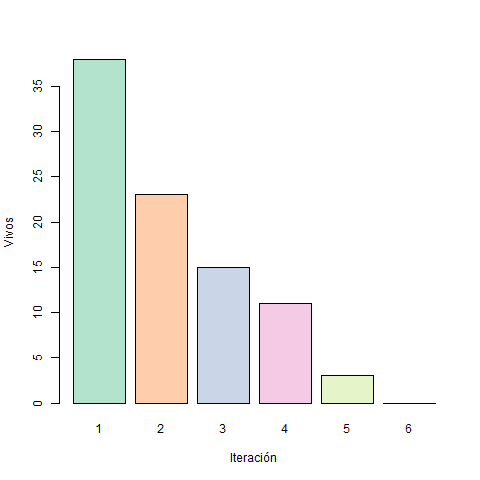
\includegraphics[width=0.5\textwidth]{regla1.png}
    \caption{\label{fig1} Diagrama de barras para la regla 1.}
    \label{fig:figura1}
\end{figure}

\begin{figure}[h!]
    \centering
    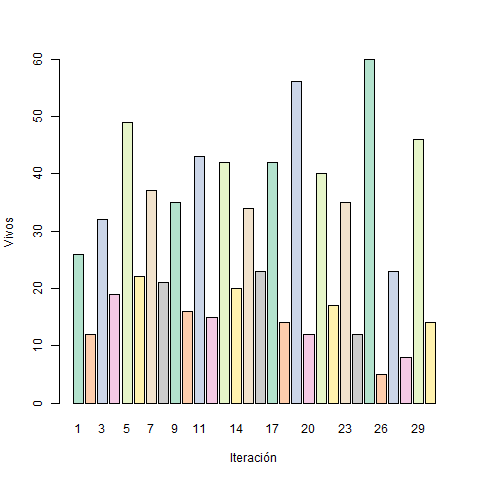
\includegraphics[width=0.5\textwidth]{regla2.png}
    \caption{\label{fig2} Diagrama de barras para la regla 2.}
    \label{fig:figura2}
\end{figure}
\bigskip
\bigskip
\bigskip

\begin{figure}[h]
    \centering
    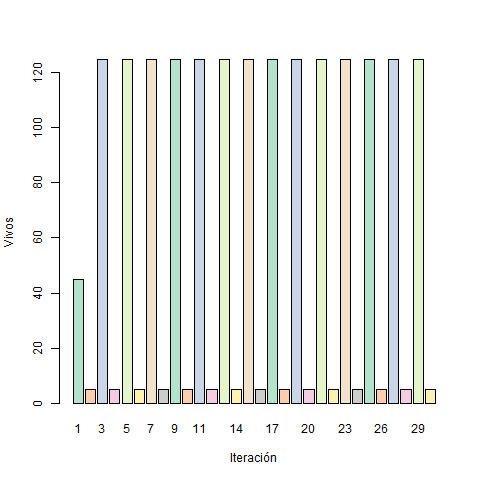
\includegraphics[width=0.5\textwidth]{regla3.png}
    \caption{\label{fig3} Diagrama de barras para la regla 3.}
    \label{fig:figura3}
\end{figure}
\bigskip
\bigskip
\bigskip

\begin{figure}[h!]
    \centering
    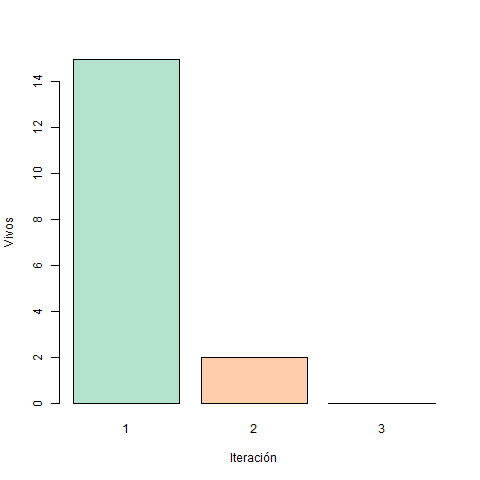
\includegraphics[width=0.5\textwidth]{regla4.png}
    \caption{\label{fig4} Diagrama de barras para la regla 4.}
    \label{fig:figura4}
\end{figure}
\bigskip

\begin{figure}[h!]
    \centering
    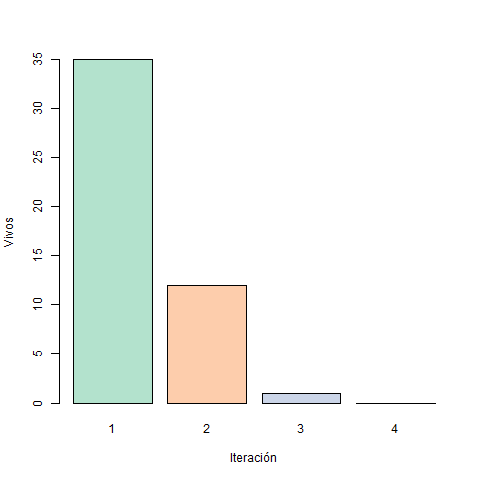
\includegraphics[width=0.5\textwidth]{regla5.png}
    \caption{\label{fig5} Diagrama de barras para la regla 5.}
    \label{fig:figura5}
\end{figure}
}
\newpage
\bibliography{Dra.Elisa}
\bibliographystyle{plainnat}


\bigskip

\end{document}



